% Author: Izaak Neutelings (March 2020)
\documentclass[border=3pt,tikz]{standalone}
\usepackage{amsmath} % for \dfrac
\usepackage{mathabx} % for \Earth
\usepackage{bm} % \bm
\usepackage{physics}
\usepackage{tikz,pgfplots}
\usepackage[outline]{contour} % glow around text
\usetikzlibrary{angles,quotes} % for pic (angle labels)
\usetikzlibrary{calc}
\usetikzlibrary{decorations.markings}
\tikzset{>=latex} % for LaTeX arrow head
\contourlength{1.6pt}
\usepackage{xcolor}
\colorlet{Bcol}{violet!90}
\colorlet{BFcol}{red!60!black}
\colorlet{veccol}{green!45!black}
\colorlet{Icol}{blue!70!black}
\tikzstyle{BField}=[->,very thick,Bcol]
\tikzstyle{current}=[->,Icol] %thick,
\tikzstyle{force}=[->,very thick,BFcol]
\tikzstyle{velocity}=[->,very thick,vcol]
\tikzstyle{charge+}=[very thin,draw=black,top color=red!50,bottom color=red!90!black,shading angle=20,circle,inner sep=0.5]
\tikzstyle{charge-}=[very thin,draw=black,top color=blue!50,bottom color=blue!80,shading angle=20,circle,inner sep=0.5]
\tikzstyle{vector}=[->,thick,veccol]
\tikzset{
  BFieldLine/.style={thick,Bcol,decoration={markings,mark=at position #1 with {\arrow{latex}}},
                     postaction={decorate}},
  BFieldLine/.default=0.5,
  pics/Bin/.style={
    code={
      \def\R{0.12}
      \draw[pic actions,Bcol,line width=0.6] % ,thick
        (0,0) circle (\R) (-135:.7*\R) -- (45:.7*\R) (-45:.7*\R) -- (135:.7*\R);
  }},
}



\begin{document}


% B FIELD horizontal, zero velocity
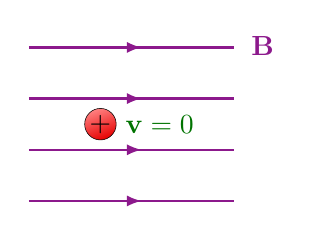
\begin{tikzpicture}
  \def\R{0.2}
  \def\NB{4}
  \def\xmax{2.6}
  \def\ymax{2.6}
  \coordinate (L) at (-0.08*\xmax,0.5*\ymax);
  \coordinate (R) at ( 1.1*\xmax,0.5*\ymax);
  \coordinate (Q) at ( 0.35*\xmax,0.5*\ymax);
  
  % MAGNETIC FIELD
  \foreach \i [evaluate={\y=(\i-0.5)*\ymax/\NB;}] in {1,...,\NB}{
    \draw[BFieldLine=0.55] (0,\y) -- (\xmax,\y);
  }
  \node[Bcol,right] at (1.04*\xmax,0.88*\ymax) {$\vb{B}$};
  
  % CHARGE
  \draw[charge+] (Q) circle (\R) node {$+$} node[right=8,veccol] {$\vb{v}=0$};
  %\node[charge+] (Q') at (Q) {$+$};
  %\node[right=6,veccol] at (Q') {$\vb{v}=0$};
  
\end{tikzpicture}


% B FIELD horizontal, velocity along
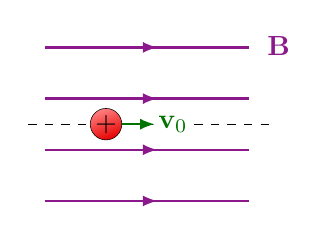
\begin{tikzpicture}
  \def\R{0.2}
  \def\v{0.16*\xmax}
  \def\NB{4}
  \def\xmax{2.6}
  \def\ymax{2.6}
  \coordinate (L) at (-0.08*\xmax,0.5*\ymax);
  \coordinate (R) at ( 1.1*\xmax,0.5*\ymax);
  \coordinate (Q) at ( 0.3*\xmax,0.5*\ymax);
  
  % MAGNETIC FIELD
  \foreach \i [evaluate={\y=(\i-0.5)*\ymax/\NB;}] in {1,...,\NB}{
    \draw[BFieldLine=0.55] (0,\y) -- (\xmax,\y);
  }
  \node[Bcol,right] at (1.04*\xmax,0.88*\ymax) {$\vb{B}$};
  
  % CHARGE
  \draw[dashed] (L) -- (R);
  \draw[vector] (Q) ++ (\R,0) --++ (\v,0) node[right=0,fill=white,inner sep=1] {$\vb{v}_0$};
  \draw[charge+] (Q) circle (\R) node {$+$};
  
\end{tikzpicture}


% B FIELD horizontal, velocity perpendicular
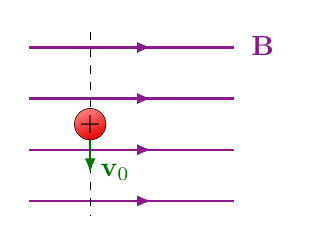
\begin{tikzpicture}
  \def\R{0.2}
  \def\v{0.16*\xmax}
  \def\NB{4}
  \def\xmax{2.6}
  \def\ymax{2.6}
  \coordinate (T) at (0.3*\xmax,0.95*\ymax);
  \coordinate (B) at (0.3*\xmax,0.05*\ymax);
  \coordinate (Q) at (0.3*\xmax,0.5*\ymax);
  
  % MAGNETIC FIELD
  \foreach \i [evaluate={\y=(\i-0.5)*\ymax/\NB;}] in {1,...,\NB}{
    \draw[BFieldLine=0.60] (0,\y) -- (\xmax,\y);
  }
  \node[Bcol,right] at (1.04*\xmax,0.88*\ymax) {$\vb{B}$};
  
  % CHARGE
  \draw[dashed] (T) -- (B);
  \draw[vector] (Q) ++ (0,-\R) --++ (0,-\v) node[right=0] {$\vb{v}_0$};
  \draw[charge+] (Q) circle (\R) node {$+$};
  
\end{tikzpicture}


% B FIELD horizontal, top view
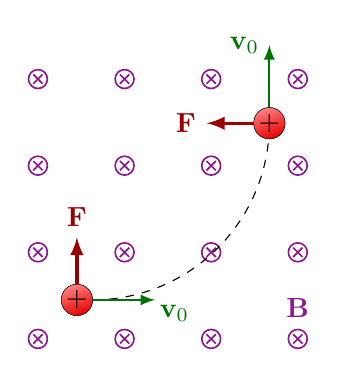
\begin{tikzpicture}
  \def\xmax{3.3}
  \def\ymax{3.3}
  \def\R{0.2}
  \def\P{0.68*\xmax}
  \def\v{0.24*\xmax}
  \def\F{0.18*\xmax}
  \def\NBy{4}
  \def\NBx{4}
  \coordinate (Q) at (0.15*\xmax,0.15*\ymax);
  
  % MAGNETIC FIELD
  \foreach \i [evaluate={\y=(\i-1)*\ymax/(\NBy-1);}] in {1,...,\NBy}{
    \foreach \i [evaluate={\x=(\i-1)*\xmax/(\NBx-1);}] in {1,...,\NBx}{
      \pic[rotate=-90] at (\x,\y) {Bin};
    }
  }
  \node[Bcol] at (\xmax,0.12*\ymax) {$\vb{B}$};
  
  % CHARGE
  \draw[dashed] (Q)++(\R,0) arc (-90:0:\P) coordinate (F);
  \draw[vector] (Q)++(\R,0) --++ (\v,0) node[below right=-2] {$\vb{v}_0$};
  \draw[vector] (F)++(0,\R) --++ (0,\v) node[left=0] {$\vb{v}_0$};
  \draw[force]  (Q)++(0,\R) --++ (0,\F) node[above=0] {$\vb{F}$};
  \draw[force]  (F)++(-\R,0) --++ (-\F,0) node[left=0] {$\vb{F}$};
  \draw[charge+] (Q) circle (\R) node {$+$};
  \draw[charge+] (F) circle (\R) node {$+$};
  
\end{tikzpicture}


% B FIELD horizontal, top view, circle
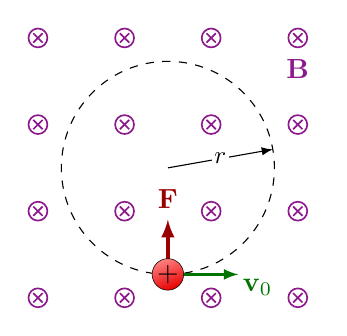
\begin{tikzpicture}
  \def\xmax{3.3}
  \def\ymax{3.3}
  \def\R{0.2}
  \def\P{0.41*\xmax}
  \def\v{0.21*\xmax}
  \def\F{0.15*\xmax}
  \def\NBy{4}
  \def\NBx{4}
  \coordinate (O) at (0.5*\xmax,0.09*\ymax+\P);
  \coordinate (Q) at (0.5*\xmax,0.09*\ymax);
  
  % MAGNETIC FIELD
  \foreach \i [evaluate={\y=(\i-1)*\ymax/(\NBy-1);}] in {1,...,\NBy}{
    \foreach \i [evaluate={\x=(\i-1)*\xmax/(\NBx-1);}] in {1,...,\NBx}{
      \pic[rotate=-90] at (\x,\y) {Bin};
    }
  }
  \node[Bcol] at (\xmax,0.88*\ymax) {$\vb{B}$};
  
  % CHARGE
  \draw[dashed] (Q) arc (-90:270:\P) coordinate (F);
  \draw[vector] (Q)++(\R,0) --++ (\v,0) node[below right=-2] {$\vb{v}_0$};
  \draw[force]  (Q)++(0,\R) --++ (0,\F) node[above=0] {$\vb{F}$};
  \draw[charge+] (Q) circle (\R) node {$+$};
  \draw[->] (O) --++ (10:\P) node[midway,fill=white,inner sep=1,scale=0.9] {$r$};
  
\end{tikzpicture}


% B FIELD horizontal, velocity along
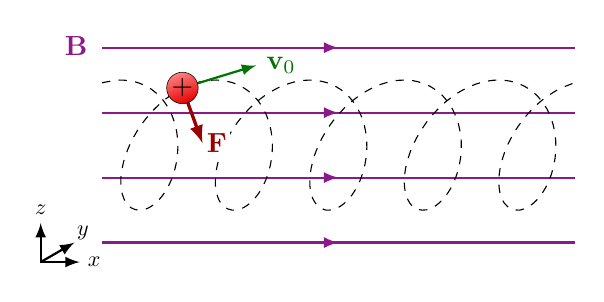
\begin{tikzpicture}[x={(1,0)},y={(0,1)},z={(0.8,0.3)}]
  \def\R{0.2}
  \def\v{0.13*\xmax}
  \def\A{0.24*\ymax}
  \def\k{300}
  \def\NB{4}
  \def\xmax{6.0}
  \def\ymax{3.3}
  \coordinate (O) at (-0.13*\xmax,0.05*\ymax);
  \coordinate (Q) at (0.17*\xmax,0.72*\ymax);
  
  \draw[->,thick] (O) --++ (30:0.15*\ymax)node[above right=-2,scale=0.8] {$y$};
  \draw[<->,thick] (O)++(0.15*\ymax,0) node[right,scale=0.8] {$x$} -- (O) --++ (0,0.15*\ymax) node[above,scale=0.8] {$z$};
  
  % MAGNETIC FIELD
  \foreach \i [evaluate={\y=(\i-0.5)*\ymax/\NB;}] in {1,...,\NB}{
    \draw[BFieldLine] (0,\y) -- (\xmax,\y);
  }
  \node[Bcol,left] at (-0.01*\xmax,0.88*\ymax) {$\vb{B}$};
  
  %\draw[->] (O) --++ (0,0,1);
  %\draw[->] (O) --++ (0,1,0);
  %\draw[->] (O) --++ (1,0,0);
  
  % CHARGE
  \draw[dashed,samples=120,smooth,variable=\x,domain=0:\xmax]
    plot(\x,{\ymax/2+\A*cos(\k*\x)},{\A*sin(\k*\x)});
  \draw[force] (Q) ++ (-70:\R) --++ (-70:0.7*\v) node[right=0,fill=white,inner sep=1] {$\vb{F}$};
  \draw[vector] (Q) ++ (17:\R) --++ (17:\v) node[right=0] {$\vb{v}_0$}; %,fill=white,inner sep=1
  \draw[charge+] (Q) circle (\R) node {$+$};
  
\end{tikzpicture}


% B FIELD vertical, velocity perpendicular, 3D
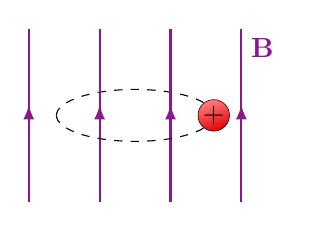
\begin{tikzpicture}
  \def\R{0.2}
  \def\W{2.7}
  \def\H{2.2}
  \def\Rx{0.37*\W}
  \def\Ry{0.15*\H}
  \def\v{0.13*\W}
  \def\NB{4}
  \coordinate (O) at (-0.13*\W,0.05*\H);
  \coordinate (Q) at (\Rx,0);
  
  % MAGNETIC FIELD
  \draw[dashed]
    (-\Rx,0) arc (180:0:{\Rx} and {\Ry});
  \foreach \i [evaluate={\x=-\W/2+(\i-1)*\W/(\NB-1);}] in {1,...,\NB}{
    \draw[BFieldLine=0.56] (\x,-\H/2) -- (\x,\H/2);
  }
  \node[Bcol,below right] at (0.5*\W,0.5*\H) {$\vb{B}$};
  
  % CHARGE
  \draw[dashed]
    (-\Rx,0) arc (180:360:{\Rx} and {\Ry});
%  \draw[force] (Q) ++ (-70:\R) --++ (-70:0.7*\v) node[right=0,fill=white,inner sep=1] {$\vb{F}$};
%  \draw[vector] (Q) ++ (17:\R) --++ (17:\v) node[right=0] {$\vb{v}_0$}; %,fill=white,inner sep=1
  \draw[charge+] (Q) circle (\R) node {$+$};
  
\end{tikzpicture}


\end{document}
